\documentclass[11pt,a4paper]{article}
\usepackage[utf8]{inputenc}
\usepackage{graphicx}
\usepackage{hyperref}
\usepackage{booktabs}
\usepackage{listings}
\usepackage{xcolor}
\usepackage{geometry}
\usepackage{amsmath}
\usepackage{listings}
\usepackage{xcolor}

\lstset{
  language=Python,
  basicstyle=\ttfamily\small,
  keywordstyle=\color{blue},
  stringstyle=\color{orange},
  commentstyle=\color{gray},
  showstringspaces=false,
  breaklines=true
}

\geometry{margin=1in}

\title{Text-Driven Market Movement Prediction\\
\large Final Project Report}
\author{Zitian}
\date{June 2025}

\begin{document}
\maketitle

\begin{abstract}
This study examines the predictive power of daily financial news headlines for next-day S\&P 500 movements. We implemented a fully managed AWS pipeline—leveraging S3 for storage, Glue for ETL, Athena for SQL querying, and SageMaker for modeling—to extract both lexicon-based and FinBERT-derived sentiment features from headlines spanning 2008–2024. We benchmarked a range of models, including LSTM (regression and classification), logistic regression, tree-based ensembles (XGBoost, Gradient Boosting, Random Forest), and LightGBM under a 5-fold time-series split. All classifiers achieved AUCs between 0.50 and 0.52 and accuracies near 0.5, indicating minimal predictive signal in daily headlines alone. These results highlight both the challenges of news-driven market prediction and the effectiveness of an end-to-end cloud-native analytics workflow.
\end{abstract}
    

\section{Introduction}
Predicting equity market moves from unstructured text is challenging yet appealing. We use a Kaggle dataset pairing S\&P\,500 closing prices with SEC headlines (2008–2024) and a financial sentiment lexicon. Our goal: build an AWS-powered pipeline to extract daily sentiment features, train classifiers, and evaluate predictive power.

\section{Data Sources}
\begin{itemize}
  \item \textbf{News \& Price Dataset} \\
    Contains date, headlines, closing price (\texttt{cp}), and next-day return.
  \item \textbf{Financial Sentiment Lexicon} \\
    Lists financial terms with sentiment scores in $[-1,1]$.
\end{itemize}

\subsection{AWS Infrastructure}

Below we describe each major stage in our AWS workflow, its purpose, and how it was implemented.

\subsubsection{S3 Buckets and Data Ingestion}

We rely on four dedicated S3 buckets:textdataproject-raw-snpnews-zitian,textdataproject-raw-lexicon-zitian, textdataproject-processed-features-zitian,textdataproject-query-results-zitian. To organize every stage of our pipeline. The first two ("raw") buckets hold the original Kaggle CSV and ZIP files for news headlines and the financial sentiment lexicon immediately after download via the AWS CLI (configured with our \texttt{TextDataProjectRole} in the Stockholm region). The "processed-features" bucket stores the Parquet outputs generated by Glue ETL jobs (daily sentiment metrics, tokenized headlines, etc.), and the "query-results" bucket is used by Athena as its query staging location. This structure ensures clear separation between raw inputs, intermediate feature tables, and analytical query outputs, all within the same region for optimal performance and security.  


\subsubsection{IAM Roles and Permissions}

To enforce least-privilege access across our data pipeline, we defined a single IAM role, \texttt{TextDataProjectRole}, which is assumed by AWS Glue, Athena, and QuickSight. Its trust policy explicitly permits the Glue, Athena, and QuickSight service principals to assume the role. In addition, we created individual IAM users with programmatic access keys mapped to this role for local development, ensuring that CLI operations and CI/CD pipelines inherit the same controlled permissions.  


\subsubsection{Glue Crawler and Data Catalog}

We set up a Glue Crawler ("raw-news-crawler") to scan our raw S3 bucket (textdataproject‐raw) on demand and automatically infer the schema of the uploaded CSVs, registering the resulting table directly into the Glue Data Catalog under the database \texttt{sentiment\_db} with the prefix \texttt{raw\_news\_}. The crawler runs under the \texttt{TextDataProjectRole}, which grants it access to S3 and the Data Catalog. Once executed, it produced the table \texttt{sentiment\_db.raw\_news\_table}, making the raw headlines and price data immediately queryable via Athena and downstream ETL jobs.  


\subsubsection{Glue ETL / CTAS to Parquet}

To optimize query performance and support analytics at scale, we transformed the raw CSV tables into columnar Parquet files and materialized our daily feature table in S3. This was accomplished in two interchangeable ways: either by running a Glue ETL job— based on the default PySpark script template— which reads from \texttt{sentiment\_db.raw\_news\_table} and writes out Parquet partitions to our processed-features bucket, or by issuing an Athena CTAS statement that selects from the raw table and writes directly in Parquet format to s3://textdataproject-processed-features-v2/. In both cases we confirmed that the output files appeared under the expected S3 path, ready for downstream querying and analysis.  

\subsubsection{Athena Query Configuration}

To provide interactive, serverless SQL access over our Parquet feature tables and to feed downstream dashboards and notebooks, we configured Athena with a dedicated results bucket in the same region. After pointing Athena's query result location to \texttt{s3://textdataproject-query-results/} in \texttt{eu-west-1}, we verified connectivity by listing tables in \texttt{sentiment\_db} and sampling rows from \texttt{daily\_features\_v2}. This setup ensures all query outputs and metadata are stored centrally, simplifying auditability and reuse across the project.  

\subsubsection{QuickSight Dashboard Integration}

We set up an Amazon QuickSight dashboard to visualize daily sentiment metrics alongside price movements, sourcing data directly from our Athena view \texttt{v\_daily\_full\_features} (with SPICE ingestion enabled for performance) under the \texttt{TextDataProjectRole}. The dashboard includes four concise visuals:

\begin{enumerate}
  \item \textbf{Daily Price vs. Sentiment:} dual‐axis line chart for closing price and lexicon/FinBERT sentiment.  
  \item \textbf{Quarterly Sentiment Trends:} grouped bar chart comparing lexicon total, average, dispersion, and FinBERT sentiment.  
  \item \textbf{Sentiment vs. Next‐Day Return:} scatter plot of daily sentiment against next‐day return with trendline.  
  \item \textbf{Sentiment Decile Returns:} bar charts showing average next‐day return per sentiment decile for both lexicon and FinBERT scores.  
\end{enumerate}

\begin{center}
  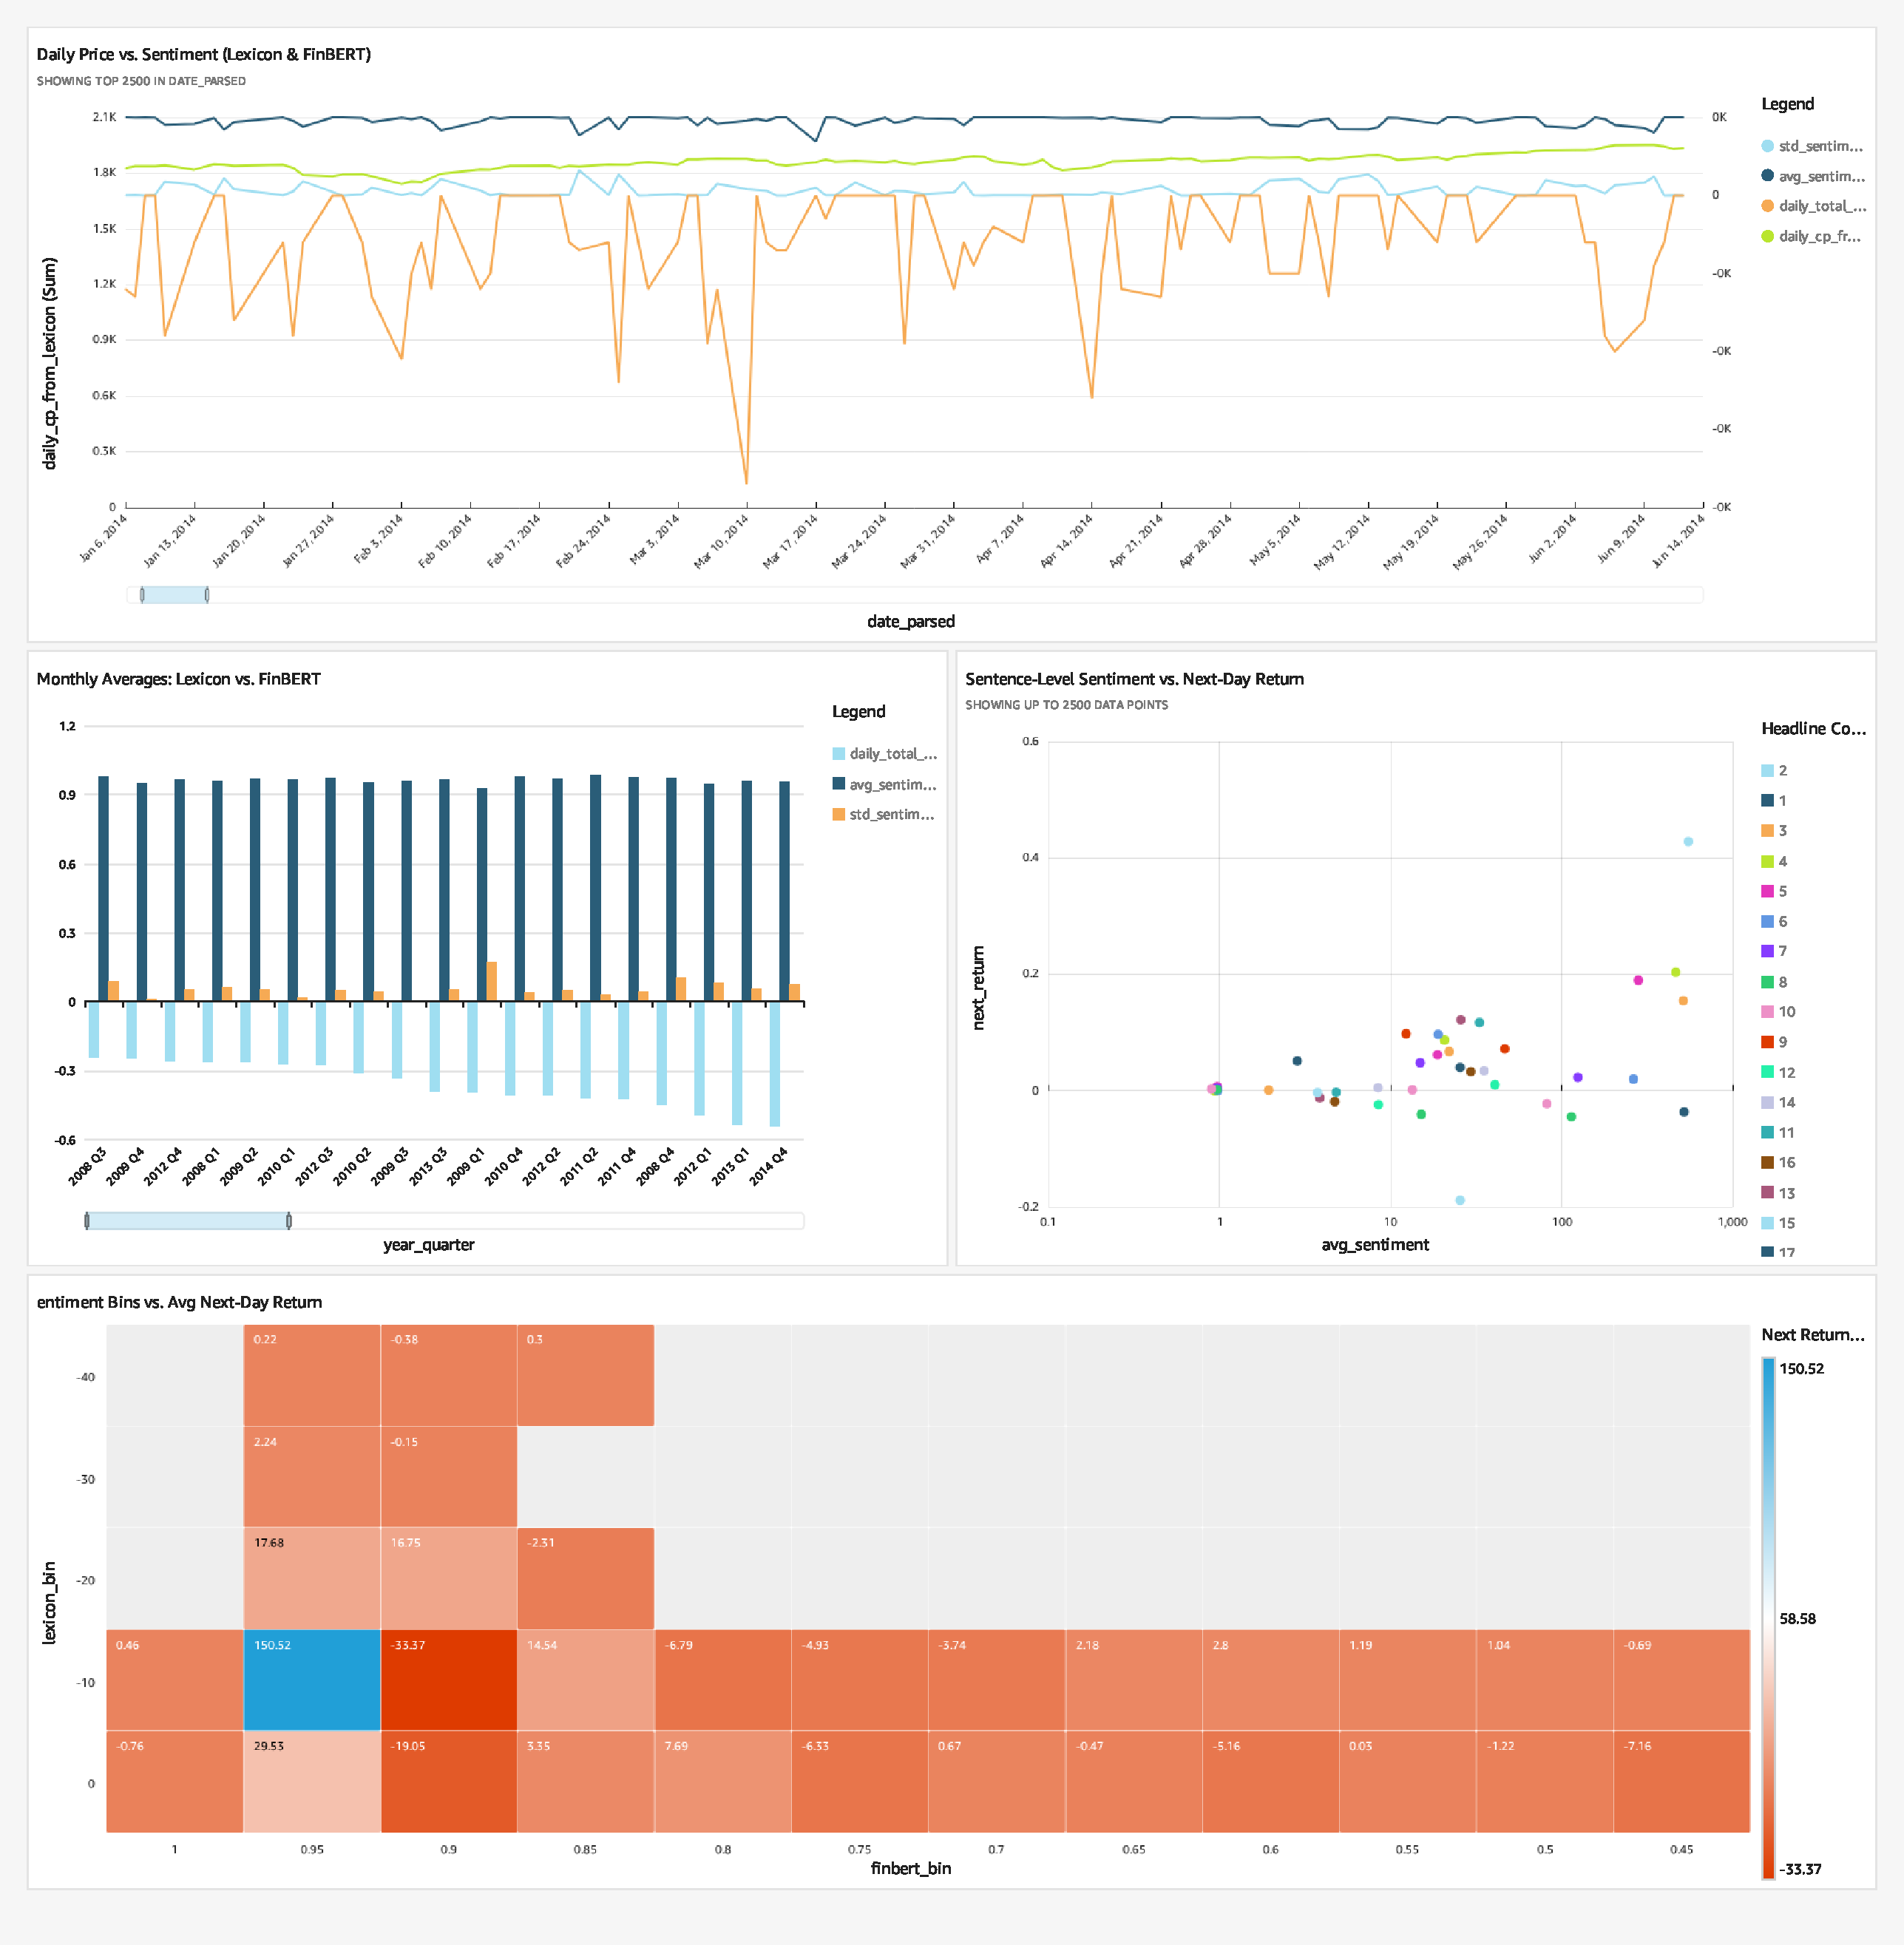
\includegraphics[width=0.85\linewidth]{dashboard_screenshot.pdf}
\end{center}


\subsection{Local Enhancement with Pandas}

Once the daily Parquet files were available in S3, we used a SageMaker notebook to compute two complementary sentiment feature sets:

\begin{enumerate}
  \item \textbf{Lexicon‐Based Token Scoring:}
  \begin{itemize}
    \item Loaded each day's headlines into a Pandas DataFrame.
    \item Tokenized headlines using simple whitespace splitting and normalized to lowercase.
    \item Merged tokens with our financial sentiment lexicon CSV (columns \texttt{word\_or\_phrase}, \texttt{sentiment\_score}).
    \item For each date, computed:
      \begin{itemize}
        \item \texttt{daily\_total\_score} = sum of matched token scores;
        \item \texttt{avg\_sentiment} = mean of token scores;
        \item \texttt{std\_sentiment} = standard deviation of token scores (filled to 0 if only one token or one headline);
        \item \texttt{daily\_pos\_count} / \texttt{daily\_neg\_count} = counts of tokens with positive / negative scores.
      \end{itemize}
  \end{itemize}

  \item \textbf{FinBERT Sentence‐Level Analysis:}
  \begin{itemize}
    \item Initialized the Hugging Face pipeline:
      \begin{lstlisting}[language=python]
from transformers import AutoTokenizer, AutoModelForSequenceClassification, pipeline
tokenizer = AutoTokenizer.from_pretrained("yiyanghkust/finbert-tone")
model     = AutoModelForSequenceClassification.from_pretrained("yiyanghkust/finbert-tone")
finbert   = pipeline("sentiment-analysis", model=model, tokenizer=tokenizer, return_all_scores=True)
      \end{lstlisting}
    \item Applied \texttt{finbert} to each raw headline to retrieve probabilities for \texttt{positive}, \texttt{neutral}, and \texttt{negative}.
    \item For each date, aggregated:
      \begin{itemize}
        \item \texttt{finbert\_pos\_mean}, \texttt{finbert\_neg\_mean}: mean positive / negative probability;
        \item \texttt{finbert\_pos\_std},  \texttt{finbert\_neg\_std}: standard deviation of those probabilities.
      \end{itemize}
  \end{itemize}
\end{enumerate}

These sentiment features were then merged with daily price data (\texttt{daily\_cp\_from\_lexicon}, \texttt{next\_return}) and extended with simple time‐series derivatives (\texttt{prev\_return\_pct}, \texttt{ma3\_return\_pct}) to construct the final modeling dataset.  


\section{Correlation Analysis of Features vs. Next-Day Return}

To assess linear relationships between our engineered sentiment features and the target variable (\texttt{next\_return}), we computed the pairwise Pearson correlation coefficients and visualized them in a heatmap (Figure~\ref{fig:correlation-heatmap}).

\begin{figure}[h]
  \centering
  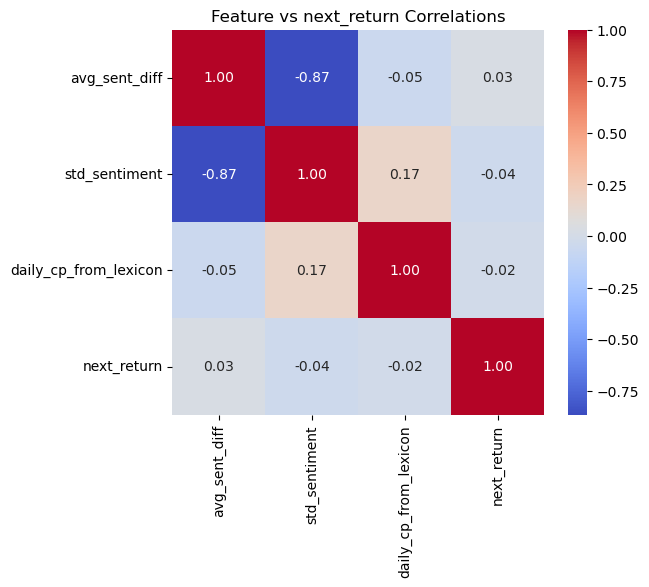
\includegraphics[width=0.5\linewidth]{output.png}
  \caption{Pearson correlation matrix.}
  \label{fig:correlation-heatmap}
\end{figure}

As shown, all off-diagonal correlations with \texttt{next\_return} are very close to zero (–0.04 to +0.03), indicating almost no linear association between any single sentiment or price feature and the subsequent return. This low degree of linear dependence suggests that simple linear models may struggle to predict price movements from these features alone, motivating our exploration of non-linear and more complex modeling approaches in subsequent sections.


\section{Modeling}

Given the near-zero linear correlations observed, we focused on non-linear classifiers under a 5-fold \texttt{TimeSeriesSplit} scheme to respect temporal ordering. Table~\ref{tab:model-results} summarizes the mean performance metrics for each model.

\begin{table}[h]
\centering
\caption{Mean classification performance over 5 folds}
\label{tab:model-results}
\begin{tabular}{lccc}
\toprule
\textbf{Model}                & \textbf{AUC} & \textbf{Accuracy} & \textbf{F1 Score} \\
\midrule
Logistic Regression (L2)      & 0.513        & 0.525             & 0.634             \\
Gradient Boosting             & 0.502        & 0.471             & 0.376             \\
Random Forest                 & 0.502        & 0.494             & 0.490             \\
XGBoost                       & 0.508        & 0.505             & 0.499             \\
LightGBM                      & 0.522        & 0.512             & 0.565             \\
\bottomrule
\end{tabular}
\end{table}

Overall, despite using sophisticated non-linear algorithms, performance remained close to random guessing. This suggests that daily headline sentiment alone—especially given sparse daily counts and simplistic lexicon or sentence-level scores—does not contain sufficient signal to predict next-day S\&P~500 movements.


\section{Results \& Discussion}

Our end-to-end AWS pipeline successfully ingested raw headlines, engineered both lexicon-based and FinBERT-derived sentiment features, and benchmarked a suite of non-linear classifiers. Table~\ref{tab:model-results} shows that the best performer—LightGBM—reached a mean AUC of 0.522, with accuracy 0.512 and F1 of 0.565. All other models hovered near chance level (AUC 0.502–0.513, accuracy 0.471–0.525), confirming that daily headline sentiment alone carries very weak predictive signal.

\begin{itemize}
  \item \textbf{Data Sparsity and Noise:} Many trading days have only one or no headline, so lexicon and FinBERT scores are based on extremely limited text.  
  \item \textbf{Coarse Sentiment Aggregation:} Simple token‐sum and sentence‐mean approaches may wash out important nuances, especially when headlines vary greatly in length and specificity.  
  \item \textbf{Lack of Contextual Market Features:} Without incorporating price momentum, volatility measures, or macroeconomic controls, sentiment features cannot be interpreted in market context.  
  \item \textbf{Measurement Error in Labels:} Next-day return is influenced by many factors (earnings releases, global events) beyond headline text; our binary up/down label may be too noisy for text-only models.
\end{itemize}

\noindent
Although the LightGBM baseline slightly outperformed random guessing, its modest AUC (0.522) suggests that richer textual representations (e.g.\ transformer embeddings), multi-day context windows, and integration of technical/fundamental indicators are necessary to unlock any significant predictive power in financial news sentiment.



\end{document}
